\section{Ziel}
Das Ziel dieses Versuchs ist es, ein Verständnis für die Funktionsweise von Operationsverstärkern zu entwickeln, indem grundlegende Schaltungen aufgebaut werden.
Es werden einige Anwendungen verwirklicht und so überprüft, dass der Operationsverstärker in Schaltungen als Integrator, Differenzierer, Schalter sowie Signalgenerator verwendet werden kann.
%Es sollen einige Anwendungen verwirklicht werden und so Unterschiede zwischen realen und idealen Operationsverstärkern bestimmt werden.


\section{Theorie}

\subsection{Operationsverstärker}
Ein Operationsverstärker (wie in \autoref{fig:OPV} zu sehen) ist ein gleichstromgekoppelter Differenzverstärker, dessen Ausgangsspannung $U_\text{A}$ proportional zur Differenz der beiden Eingangsspannungen $U_\text{P}$ und $U_\text{N}$ ist
\begin{equation*}
    U_\text{A} = V_0 (U_\text{P} - U_\text{N}) \, .
\end{equation*}
Dabei ist $V_0$ die Leerlaufverstärkung des Operationsverstärkers. Bei einem idealen Operationsverstärker ist die Leerlaufverstärkung unendlich, während sie bei einem realen Werte von etwa $\num{200000}$ \cite{Verstaerkung} erreicht und frequenzabhängig ist.

Es gibt einen nicht-invertierenden und einen invertierenden Eingang, bei welchem die Spannung gegenphasig zur Ausgangsspannung ist. Die Eingangswiderstände sind bei einem idealen Operationsverstärker unendlich und für einen realen sehr groß. Der Ausgangswiderstand ist idealerweise Null. Ein realer Operationsverstärker hat einen sehr kleinen Ausgangswiderstand.

\begin{figure}
    \centering
    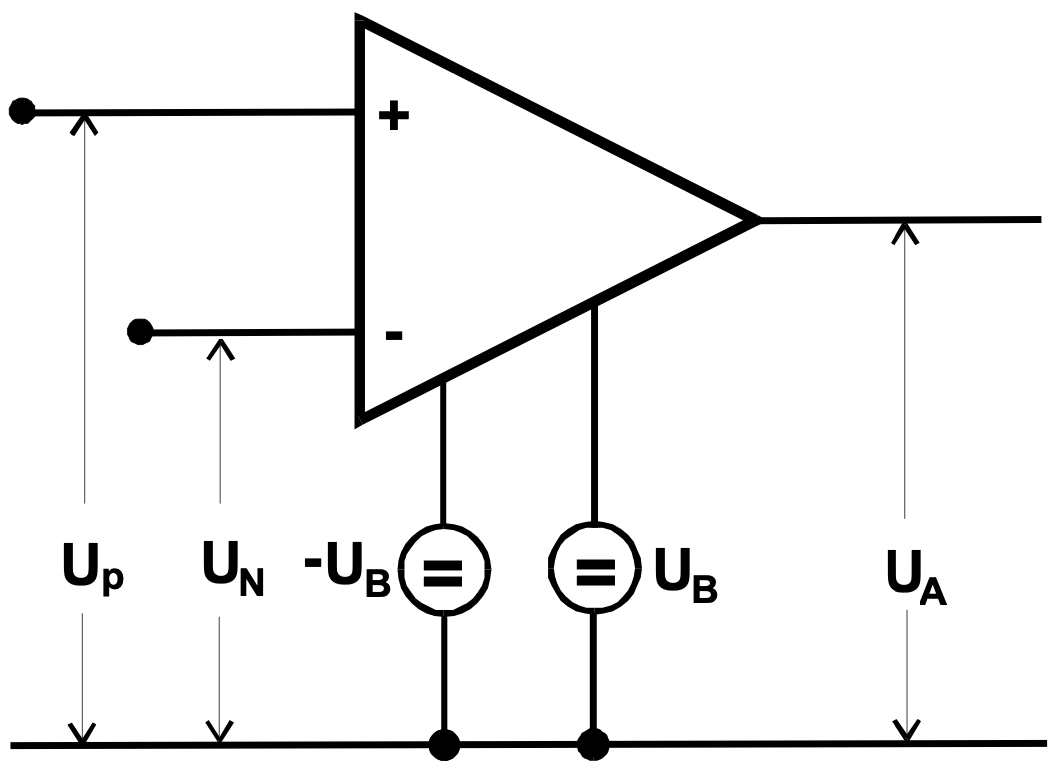
\includegraphics[width=0.5\linewidth]{./figures/OPV.png}
    \caption{Das Schaltsymbol eines Operationsverstärkers. Es sind die beiden Eingangsspannungen $U_\text{P}$ (am nicht-invertierenden Eingang) und $U_\text{N}$ (am invertierenden Eingang), die Betriebsspannung $U_\text{B}$ und $-U_\text{B}$ sowie die Ausgangsspannung $U_\text{A}$ zu sehen.}
    \label{fig:OPV}
\end{figure}

%Neben den bereits genannten Kenngrößen gibt sind außerdem weitere wichtige Größen zu nennen. \dots

Die Ausgangsspannung kann maximal und minimal den Wert der Betriebsspannung $U_\text{B}$ annehmen. Die Verstärkungskennlinie ist in \autoref{fig:kennlinie} abgebildet. Der Ansteuerungsbereich des Operationsverstärkers kann wie in \autoref{sec:linearverstaerker} beschrieben vergrößert werden.

\begin{figure}
    \centering
    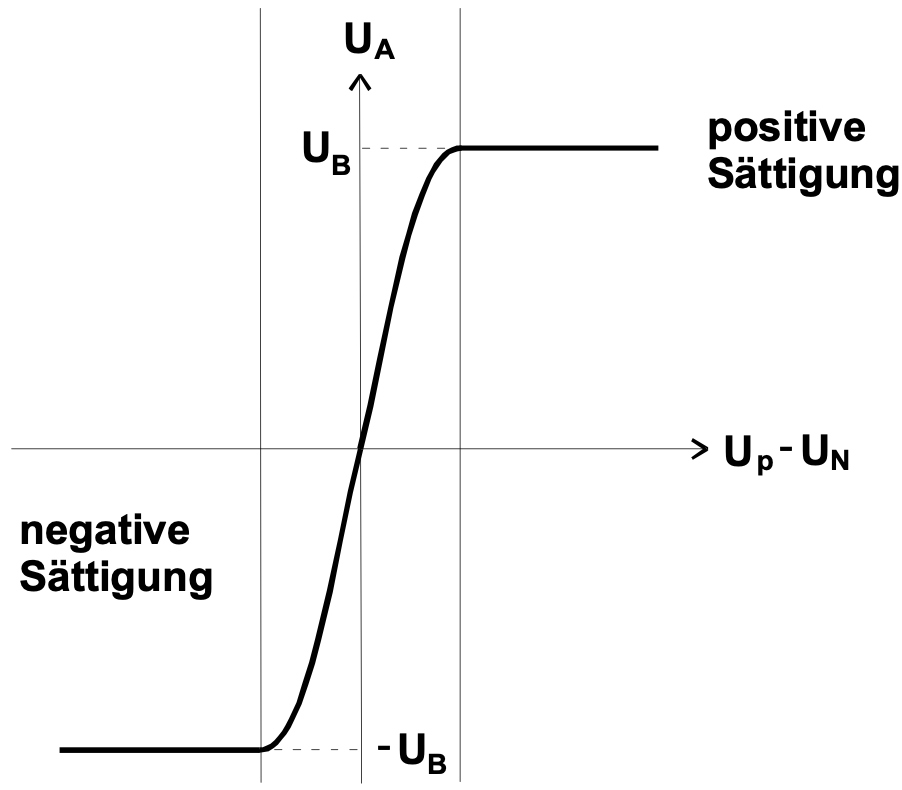
\includegraphics[width=0.5\linewidth]{./figures/Kennlinie.png}
    \caption{Die Verstärkungskennlinie eines Operationsverstärkers bei symmetrischer Betriebsspannung. Die Ausgangsspannung ist in Abhängigkeit der Differenz der Eingangsspannungen dargestellt. Außerhalb des Ansteuerungsbereichs erreicht die Ausgangsspannung einen Sättigungsbereich. \cite{V51old}} 
    \label{fig:kennlinie}
\end{figure}



\newpage
\subsection{Schaltungen mit Operationsverstärkern}
\label{sec:Schaltungen}

Im Folgenden werden einige wichtige Schaltungen und Anwendungen mit Operationsverstärkern beschrieben.

\subsubsection{Linearverstärker}
\label{sec:linearverstaerker}
Die Schaltung des invertierenden Linearverstärkers ist in \autoref{fig:InvLinear} abgebildet.

\begin{figure}
    \centering
    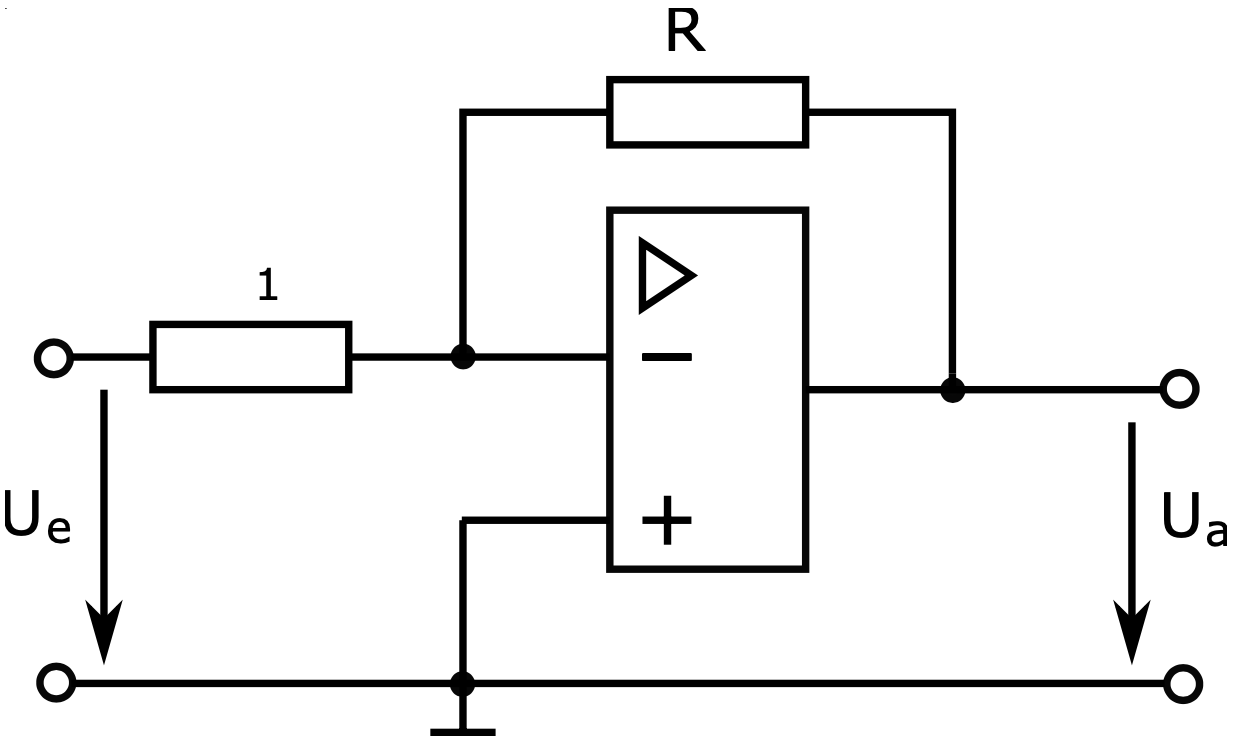
\includegraphics[width=0.7\linewidth]{./figures/1_InvLinear.png}
    \caption{Die Schaltung des invertierenden Linearverstärkers. Hier ist $U_\text{e}$ die Eingangsspannung, $U_\text{a}$ die Ausgangsspannung, R steht für den Widerstand $R_2$ und der mit 1 gekennzeichnete Widerstand ist $R_1$. \cite{V51}}
    \label{fig:InvLinear}
\end{figure}

Bei einem invertierenden Linearverstärker wird mit einer Gegenkopplung gearbeitet. Es wird ein Teil der Ausgangsspannung zurück auf den invertierenden Eingang gegeben wodurch eine Zunahme der Ausgangsspannung eine Abnahme der Eingangsspannung bedeutet. Dadurch kann der Ansteuerungsbereich vergrößert werden. Es wird also verhindert, dass bereits für eine minimale Eingangsspannungsdifferenz die Aussteuergrenze erreicht wird. Die Gesamtverstärkung der Schaltung ist kleiner als die Leerlaufverstärkung und bei einem idealen Operationsverstärker nur abhängig von dem Verhältnis der beiden Widerstände
\begin{equation*}
    V = \frac{U_\text{A}}{U_\text{E}} = - \frac{R_2}{R_1} \, .
\end{equation*}
%folgt aus der Kirchhoffscher Knotenregel; I_P = I_N = 0A, da R_E = unendlich
Durch die Gegenkopplung wird eine hohe Stabilität der Schaltung erreicht. Die Verstärkung ist auch bei Operationsverstärkern mit endlicher Leerlaufverstärkung näherungsweise nur vom Widerstandsverhältnis abhängig und somit stabil gegenüber Schwankungen der Leerlaufverstärkung, beispielsweise aufgrund von Temperaturänderungen.

Die Gegenkopplung erhöht die Bandbreite der Frequenz. Das ist in \autoref{fig:Bandbreite} zu sehen. Das Produkt der Bandbreite und der Verstärkung ist immer konstant.

\begin{figure}
    \centering
    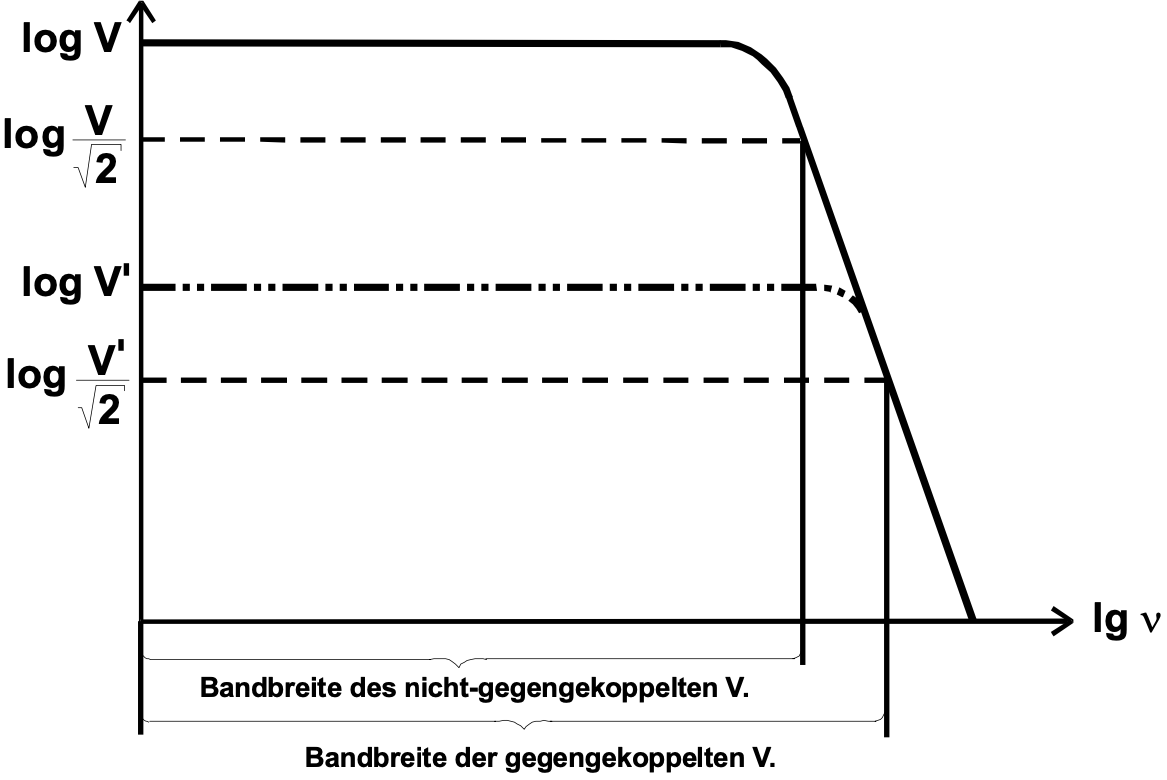
\includegraphics[width=0.7\linewidth]{./figures/Bandbreite.png}
    \caption{Die Verstärkung ist in Abhängigkeit der Frequenz $\nu$ doppellogarithmisch aufgetragen. Hier ist $V$ die Leerlaufverstärkung und $V'$ die Verstärkung mit Gegenkopplung. \cite{V51old}}
\end{figure}


\subsubsection{Umkehr-Integrator}
Ein Umkehr-Integrator integriert die Eingangsspannung.
Dafür wird in den Rückkopplungszweig ein Kondensator eingebaut. Die Schaltung ist in \autoref{fig:UmkehrInt} dargestellt.

\begin{figure}
    \centering
    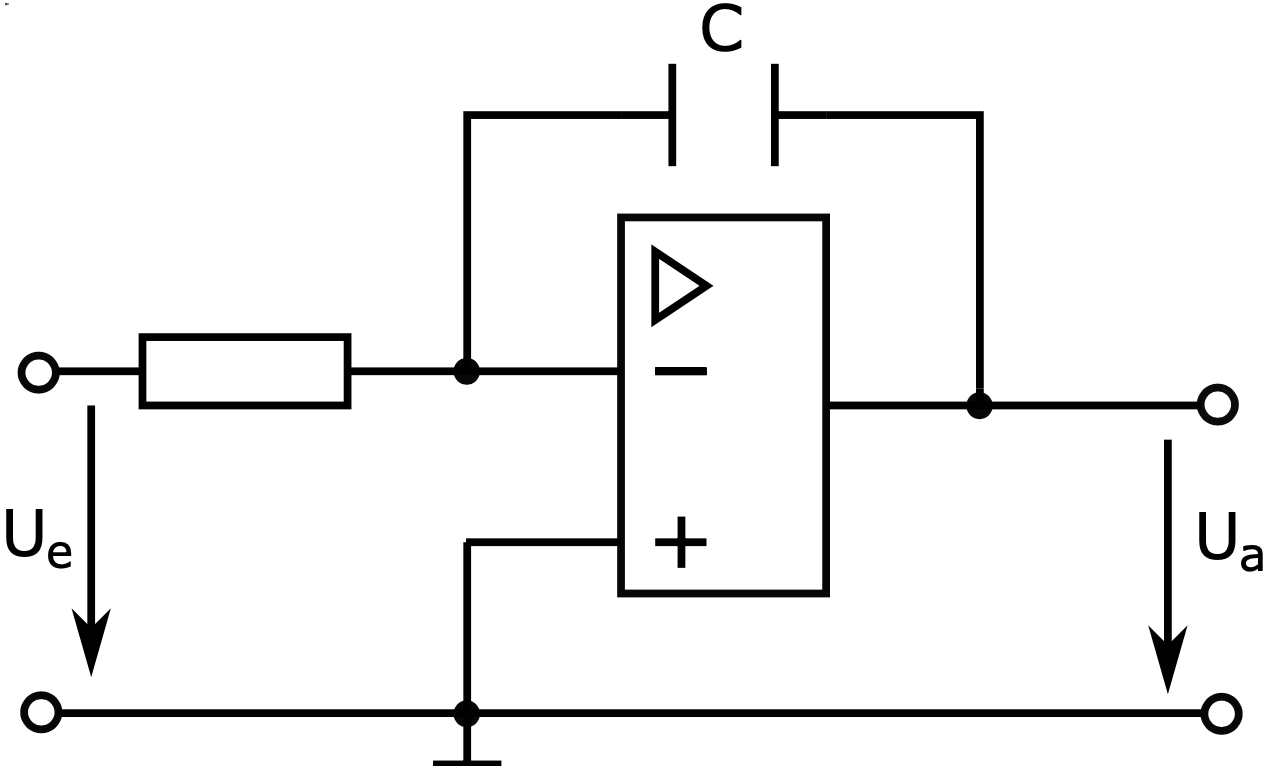
\includegraphics[width=0.7\linewidth]{./figures/2_Umkehr.png}
    \caption{Die Schaltung des Umkehr-Integrators. Der Widerstand hat den Wert $R$. Der Kondensator im Rückkopplungszweig hat die Kapazität $C$. \cite{V51}}
    \label{fig:UmkehrInt}
\end{figure}
\FloatBarrier

Am Eingang fließt kein Strom, also $I_\text{N} = 0$. Aus der Knotenregel folgt dann, dass $I_\text{R} = - I_\text{C}$ ist. Daraus ergibt sich für die Ausgangsspannung
\begin{equation*}
    U_\text{A} = - \frac{1}{R C} \int U_\text{E}(t) dt \, .
    \label{eq:Integrator}
\end{equation*}
Für ein sinusförmiges Eingangssignal
\begin{equation}
    U_\text{E} = U_0 \sin(\omega t)
    \label{eq:Sinus}
\end{equation}
ergibt sich ein kosinusförmiges Ausgangssignal, das umgekehrt proportional zur Frequenz $\omega$ ist
\begin{equation}
    U_\text{A} = \frac{U_0}{\omega R C} \cos(\omega t) \, .
    \label{eq:Int_Kosinus}
\end{equation}


\subsubsection{Umkehr-Differenzierer}
Analog zum Integrator differenziert der Umkehr-Differenzierer die Eingangsspannung. Die Schaltung ist in \autoref{fig:InvDiff} gezeigt.

\begin{figure}
    \centering
    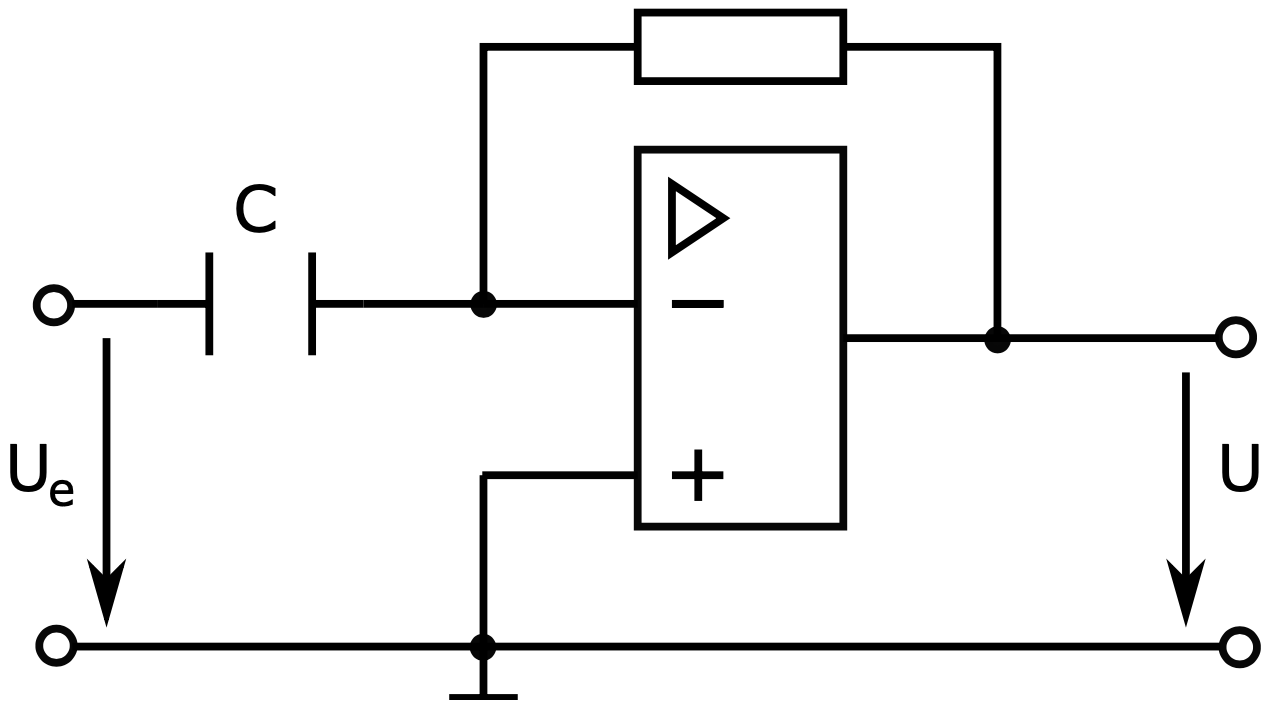
\includegraphics[width=0.7\linewidth]{./figures/3_InvDiff.png}
    \caption{Die Schaltung des Umkehr-Differenzierers. Der Kondensator hat die Kapazität $C$. In dem Rückkopplungszweig ist der Widerstand $R$ eingebaut. \cite{V51}}
    \label{fig:InvDiff}
\end{figure}
\FloatBarrier

Aus der Knotenregel folgt, dass $I_\text{C} = - I_\text{R}$ ist. Daraus folgt für die Ausgangsspannung
\begin{equation*}
    U_\text{A} = - R C \frac{d U_\text{E}}{dt} \, .
    \label{eq:Differenzierer}
\end{equation*}
Bei einem sinusförmigen Eingangssignal wie in \autoref{eq:Sinus} hat das Ausgangssignal die Form 
\begin{equation}
    U_\text{A} = - \omega R C U_0 \cos(\omega t)
    \label{eq:Diff_Kosinus}
\end{equation}
und ist, anders als beim Integrator, proportional zur Frequenz $\omega$.

\subsubsection{Schmitt-Trigger}
Eine weitere Anwendung des Operationsverstärkers ist der Schmitt-Trigger. Hier fungiert der Operationsverstärker als Schalter. Die Schaltung ist in \autoref{fig:Schmitt} abgebildet.

\begin{figure}
    \centering
    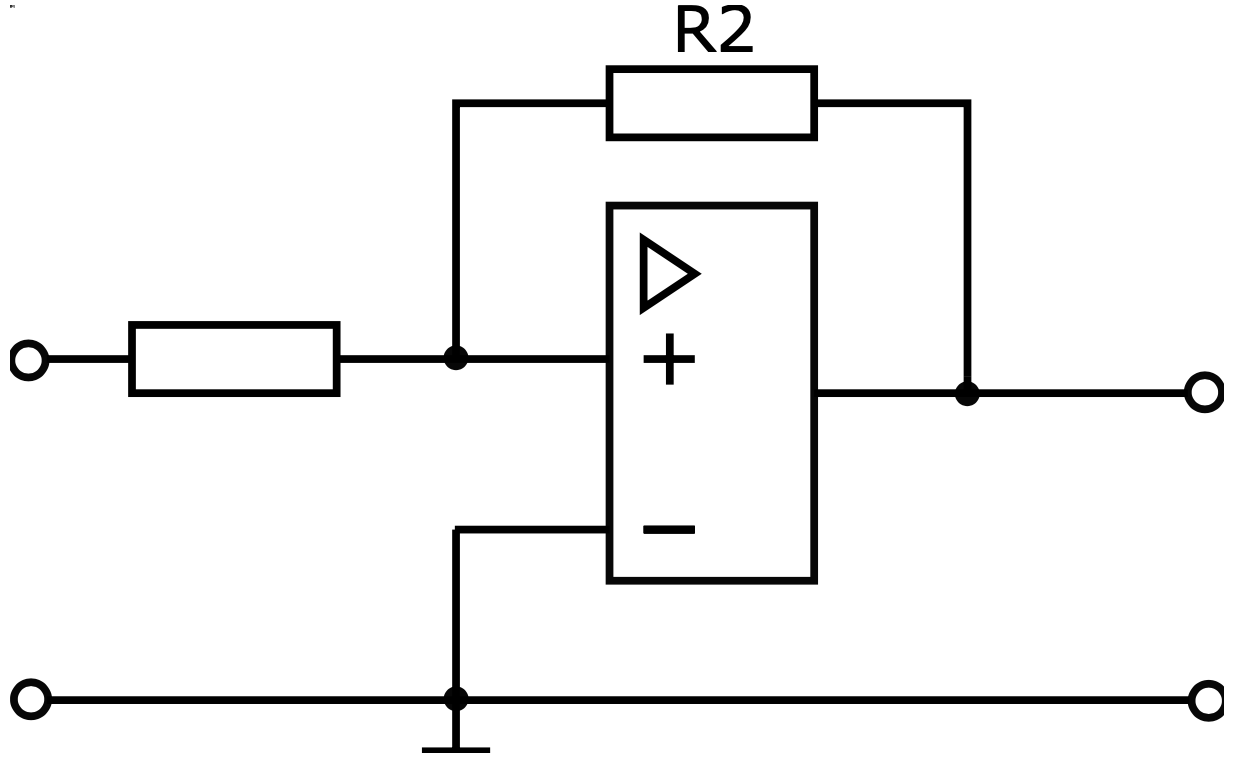
\includegraphics[width=0.7\linewidth]{./figures/4_Schmitt.png}
    \caption{Die Schaltung des Schmitt-Triggers. Der erste Widerstand hat den Wert $R_1$. Der Widerstand im Mitkopplungszweig hat den Wert $R_2$. \cite{V51}}
    \label{fig:Schmitt}
\end{figure}

Beim Schmitt-Trigger wird eine Mitkopplung verwendet. Ein Teil der Ausgangsspannung wird auf den nicht-invertierenden Eingang zurückgegeben. Bei Zunahme der Ausgangsspannung nimmt die Eingangsspannung ebenfalls zu. Das wiederum führt zu einer Zunahme der Ausgangsspannung. Die Schaltung hat also eine selbstverstärkende Wirkung.
Das Verhalten der Schaltung ist instabil. Wird eine bestimmte Schwelle erreicht, kippt die Schaltung von einem Zustand in einen anderen.

Die Schwellspannung ist durch 
\begin{equation*}
    \pm U_\text{thres} = \pm \frac{R_1}{R_2} U_\text{B}
    \label{eq:Schwelle}
\end{equation*}
definiert. Bei diesen Werten von $U_\text{E}$ wechselt die Spannung $U_\text{P}$ gerade ihr Vorzeichen.
Überschreitet die Eingangsspannung $U_\text{E}$ diesen Wert $+ U_\text{thres}$, nimmt die Ausgangsspannung den Wert der Betriebsspannung an. Unterschreitet die Eingangsspannung $- U_\text{thres}$ folgt für die Ausgangsspannung $U_\text{A} = - U_\text{B}$.

Die Verläufe eines sinusförmigen Eingangssignals und des resultierenden rechteckförmigen Ausgangssignals sind in \autoref{fig:Kurvenverlauf} zu sehen.

Wird die Ausgangsspannung in Abhängigkeit der Eingangsspannung aufgetragen, ergibt sich eine Hysterese. Diese ist in \autoref{fig:Hysterese} dargestellt. %noch mehr erklären?

\begin{figure}
    \centering
    \begin{subfigure}{0.48\textwidth}
        \centering
        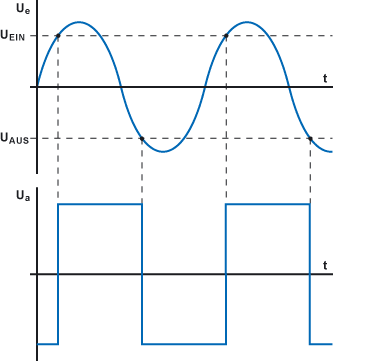
\includegraphics[width=0.75\linewidth]{./figures/Kurvenverlauf.png}
        \caption{Der Verlauf einer sinusförmigen Eingangsspannung $U_\text{E}$ und die resultierende Ausgangsspannung $U_\text{A}$ bei einer Schmitt-Trigger-Schaltung. \cite{SchmittTrigger}}
        \label{fig:Kurvenverlauf}
    \end{subfigure}
    \begin{subfigure}{0.48\textwidth}
        \centering
        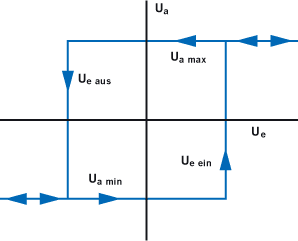
\includegraphics[width=0.8\linewidth]{./figures/Hysterese.png}
        \caption{Die Ausgangsspannung $U_\text{A}$ in Abhängigkeit der Eingangsspannung $U_\text{E}$ bei einer Schmitt-Trigger-Schaltung. \cite{SchmittTrigger}}
        \label{fig:Hysterese}
    \end{subfigure}
    \caption{Abbildungen zur Schmitt-Trigger-Schaltung.}
    \label{fig:Abbildung}
\end{figure}

\subsubsection{Signalgenerator}
Werden ein Schmitt-Trigger und ein Integrator zusammengeschaltet, ergibt sich ein Signalgenerator. Die Schaltung ist in \autoref{fig:Signal} zu sehen.

\begin{figure}
    \centering
    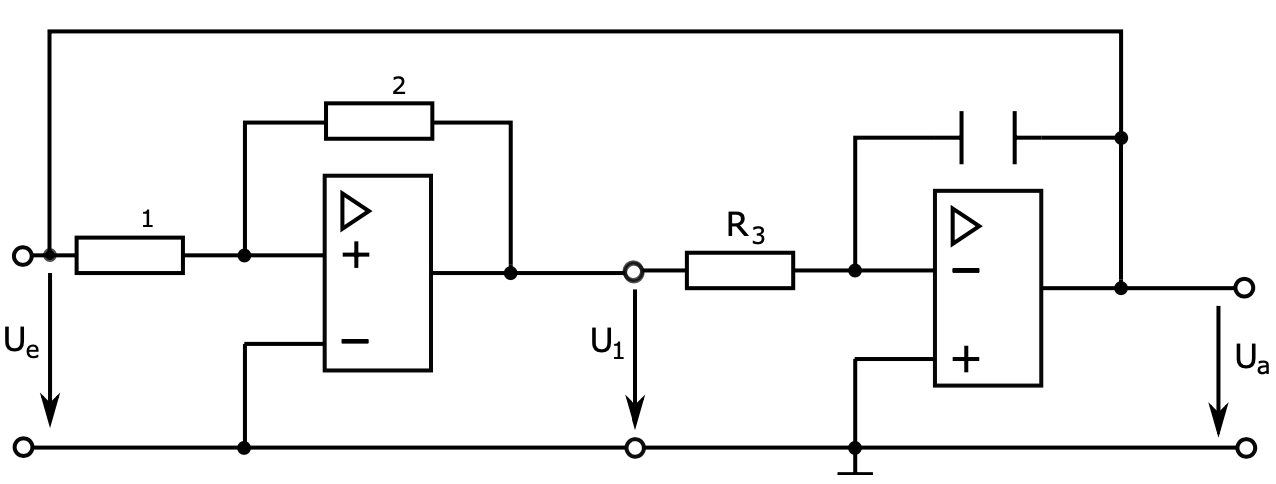
\includegraphics[width=0.7\linewidth]{./figures/5_Signal.png}
    \caption{Die Schaltung eines Signalgenerators besteht aus einer Schmitt-Trigger-Schaltung und einem Integrator. Der Ausgang des Integrator wird auf den Eingang des Schmitt-Triggers zurückgeführt. \cite{V51}}
    \label{fig:Signal}
\end{figure}

Die Ausgangsspannung des Schmitt-Triggers $U_1 = + U_\text{B}$ wird integriert. Die Ausgangsspannung des Integrators $U_\text{A}$ verringert sich mit der Zeit und erreicht die Schwelle $- R_1/R_2 U_\text{B}$. Dadurch kippt die Ausgangsspannung des Schmitt-Triggers auf $U_1 = - U_\text{B}$. Diese wird integriert, bis die Schwelle $+ R_1/R_2 U_\text{B}$ erreicht wird und die Ausgangsspannung des Schmitt-Triggers wieder auf $U_1 = + U_\text{B}$ kippt. Es ergibt sich also eine periodische Schwingung am Ausgang des Integrators in Form eines Dreiecksignals. Die Frequenz $f$ dieser Schwingung ist nur abhängig von den verwendeten Widerständen und der Kapazität
\begin{equation}
    f = \frac{R_2}{4 R_1 R_3 C} \, .
    \label{eq:Frequenz}
\end{equation}









%Formeln aus der Kurzanleitung
%\begin{equation*}
%    \nu_{Dreieck} = \frac{R_2}{4 C R_1 R_3}
%\end{equation*}

%Zu zeitlich veränderlichen Amplituden:
%\begin{align}
%    T &= 2 \pi R C \\ %Schwingungsdauer
%    \tau &= \frac{20 R C}{|\eta|} %Abklingdauer
%    \label{eq:SchwingAbkling}
%\end{align}
%Hier ist $\tau$ die Zeit für die Abnahme der Amplitude bis auf den e-ten Teil ihres Anfangswerts bzw. für die Zunahme der Amplitude auf das e-fache ihres Anfangswerts und $\eta$ die Dämpfung ($\eta < 0$) bzw. Enddämpfung ($\eta > 0$). Diese gibt den Bruchteil der Ausgangsspannung $U_A$ an, welcher auf den Eingang des OPV2 gegeben wird. %was ist das?